\section{Mon, Sep 24, 2018}

This week will feel like Hell.

Why do I feel this way? I'm not sure. I just have a feeling. Woke up with a panic
attack this morning. That's never a good sign for any week whatsoever. But I came
into work. Almost stayed home, but no I can't do that. A panic attack doesn't equate
to being sick. Anxiety runs in me. Fine. It's a fact. I cannot allow it to define who
I am.

\begin{figure}[h!]
  \centering
  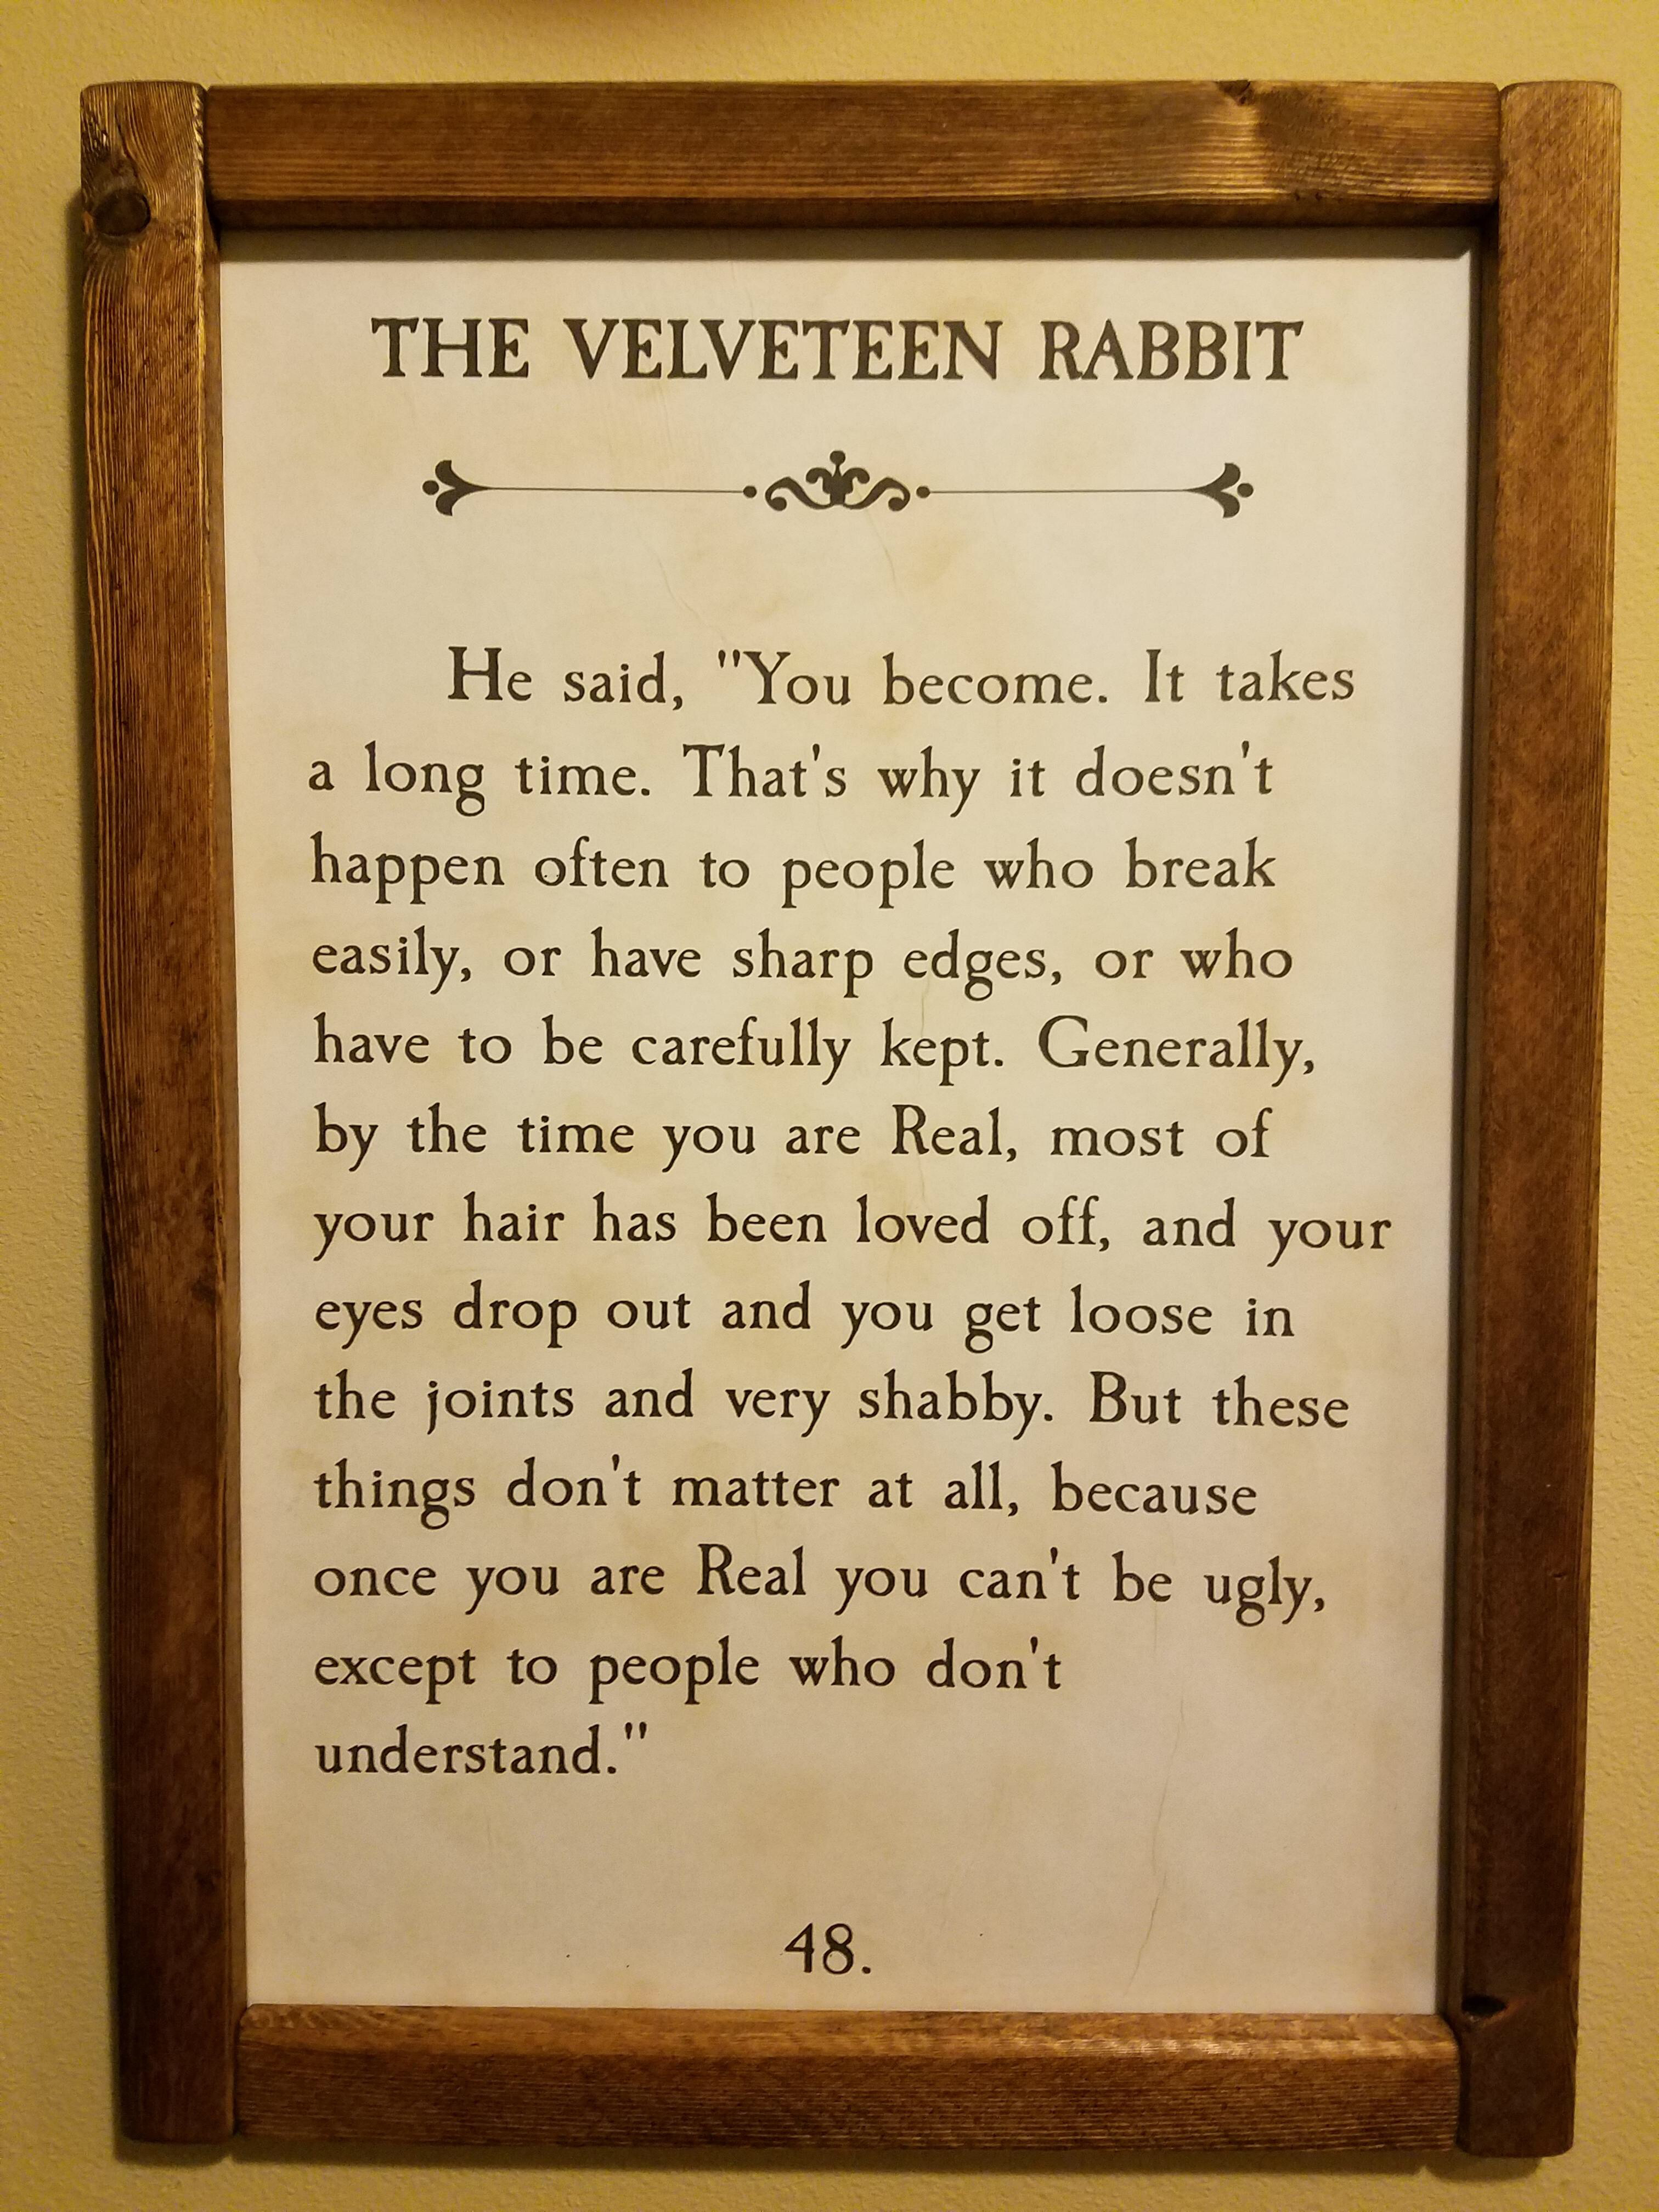
\includegraphics[width=.5\linewidth]{2018/images/rabbit.jpg}
  \caption{Velveteen Rabbit}
  \label{fig:rabbit}
\end{figure}

``He said, `You become. It takes a long time. That's why it doesn't happen often to
people who break easily, or have sharp edges, or who have to be carefully kept.
Generally, by the time you are Real, most of your hair has been loved off, and your
eyes drop out and you get loose in the joints and very shabby. But these things don't
matter at all, because once you are Real you can't be ugly, except to people who
don't understand.'"\footnote{The Velveteen Rabbit}

Ah such a life to live. Not being ugly because you think you are not. To be able to
see past anything like that would be amazing. Not a lot of people grasp that concept,
unfortunately. There are so many things in this life we wish we could understand and
hold onto. Yet we don't. It's not an easy thing at all. It is but a life sure, but we
do not know why any of that happens to us. We are but living creatures.
